\chapter{Background}

In this chapter, we provide a basic understanding of the fundamentals necessary to understand
further parts of this dissertation. First, basic Kubernetes concepts and its philosophy are
explained. Next, we describe Kubernetes' structure, including the container orchestration process.
Finally, we provide information about an important concept used in the project --- custom resources.

\section{Kubernetes Basics}
On an abstract level, a user interacts with Kubernetes by describing a desired state, which
Kubernetes then tries to enact. The actual state may be dynamically and constantly changing, for
example due to machine failures or scheduling decisions on Kubernetes' part.

Most Kubernetes objects represent stateless constructs. When deploying a stateful application, such as a
MySQL database cluster, we need to use structures designed specifically for such stateful cases. In
the latest versions of Kubernetes, we are provided with some useful stateful objects, such as
PersistentVolumes or StatefulSets.

It is useful to make a note about Kubernetes' design philosophy.
Kubernetes objects are meant to be just that --- objects. They are to represent nouns rather than
verbs. As such, we usually do not create objects that are responsible for a single action. Instead,
for example, one may create an object that represents an agent that performs the desired action
periodically.

\section{Kubernetes Architecture}

Kubernetes is a container orchestration tool. Its job is managing containers running on Pods. Pods
are the atomic units of computing used in Kubernetes --- they are an abstraction for a~set of
containers with shared resources. The real working machines, to which Pods are tied to by the
scheduler, are referred to as nodes. These work in bigger groups, so-called clusters, which
create single logical units in Kubernetes. There is one master node, responsible for orchestrating
the cluster and keeping track of state necessary to accomplish this goal. Business logic is
performed by worker nodes --- work is allocated to them dynamically to fulfill requests from users.
In the event of a node failing, the Pods on it will be recreated on a new,
working node. This ensures continuous work of cluster applications.

\begin{figure}[!ht]
    \centering
    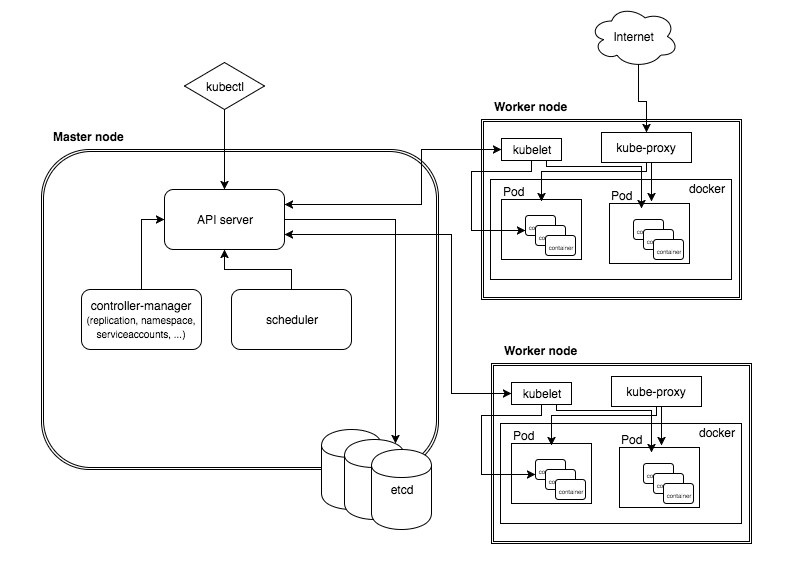
\includegraphics[width=1\textwidth, angle=0]{img/architecture.png}
    \caption{Kubernetes architecture~\cite{arch}}
    \label{fig:arch}
\end{figure}

To get a better understanding of Kubernetes' structure, let's take a look at the data presented
in Figure \ref{fig:arch}. Each worker node is equipped with a program called \textbf{kubelet},
responsible for managing Pods on that particular node, and for communication with the master. The
kube-apiserver runs on every node in order to provide TCP and UDP forwarding across the backend.

The master node is responsible for processing events in the cluster and making global decisions,
such as scheduling and scaling. It consists of several components that allow for communication
between other nodes and cluster users, such as the kube-apiserver, etcd, and kube-controller-manager.
One of the most important features of the master node is a server running on it, exposing a RESTful
API. The API may be queried by users and applications to get information about the cluster's current
state, and requests can be made to request the addition, deletion, or modification of various API
objects. As requests are made, a desired state is defined. It is the job of a group of controllers
within kube-controller-manager to make the actual state match this desired state. The master node
uses etcd to store information about the cluster's state. Requests to the Kubernetes apiserver
result in queries and modifications of the data stored in etcd.

\section{Expanding the Kubernetes API}
Kubernetes was designed to be easily extensible and configurable~\cite{extending-kubeapi}. There are
many ways of customizing the API and adding new functionalities, so called \textbf{custom resources}.

The idea behind custom resources is to allow the user to define new API objects that can be handled
in the same way as resources already understood by Kubernetes. As a result, they provide a way of
customizing a specific Kubernetes installation, exposing new behavior that can be accessed via the
same \texttt{kubectl} operations as default resources. There are two ways of defining custom resources: using
the aggregation layer or CustomResourceDefinitions.

The first way of expanding the Kubernetes API, introduced in Kubernetes 1.7, is using the
aggregation layer. Thanks to this tool, one can perform API aggregation at runtime. The aggregation
layer enables the creation of custom resources by deploying its own API server.

CustomResourceDefinitions are static objects in the API. A user can create a
CustomResourceDefinition object in the API, specifying a name and schema for the type of custom
resource they wish to introduce. Once a CustomResourceDefinition exists, custom resource objects of the defined type can
be created by users. This way of creating custom resources provides developers with less flexibility
than the aggregation layer, but requires less overhead for simple applications.

The MySQL Operator is implemented using CustomResourceDefinitions because of the simplicity and
modern design of this option. This way of extending Kubernetes API is a new concept (beta version in
Kubernetes 1.9), but it will likely be supported and extended in future versions. Though
CustomResourceDefinitions' functionalities are limited compared to the aggregation layer's, they
are suitable for our project's needs.
